\documentclass{llncs}
\usepackage[show]{ed}
\usepackage{calbf}
\usepackage{stex-logo}
\usepackage{amstext,amsmath,amssymb}
\usepackage{xspace}

\usepackage{mdframed}
\newenvironment{boxedquote}{\begin{mdframed}[leftmargin=1cm,rightmargin=1cm]}{\end{mdframed}}

\usepackage{wrapfig,paralist}
\usepackage[hyperref,style=alphabetic,backend=bibtex]{biblatex}
% \addbibresource{kwarcpubs.bib}
% \addbibresource{extpubs.bib}
% \addbibresource{kwarccrossrefs.bib}
% \addbibresource{extcrossrefs.bib}
\addbibresource{kwarc.bib}
\addbibresource{rest.bib}
\def\latexml{{\LaTeX}ML\xspace}
\pagestyle{plain}
\usepackage{tikz}\usetikzlibrary{docicon}

\usepackage{hyperref}
\title{System Description: A Semantics-Aware {\LaTeX}-to-DOCX/ODF Converter}
\author{Lukas Kohlhase and Michael Kohlhase}
\institute{Mathematics/Computer Science\\
  Jacobs University Bremen}
\begin{document}
\maketitle
\begin{abstract}
  We present a {\LaTeX}-to-Office conversion plugin for \latexml ML that can bridge the
  divide between publication practices in the theoretical disciplines (\LaTeX) and the
  applied ones (predominantly Office). The advantage of this plugin over other converters
  is that \latexml conserves enough of the document- and formula structure, that the
  transformed structures can be edited and processed further.
\end{abstract}

\section{Problem \& State of the Art}\label{sec:intro}

Many researchers in STEM fields only use {\LaTeX} to typeset their documents. However many
people still use Microsoft Word/Open office exclusively for their typesetting. When these
two groups of people intersect, it can lead to friction, as transforming text to {\LaTeX}
is quite trivial but not the opposite. For example if a conference requested documents in
Word format, the only recourse is often to just write the document in Word, which is a
pain, especially if any Mathematics is to be included.

\ednote{Here we state the Problem, some conferences and admin want papers in word format,
  however LaTeX is superior for various reasons. Hence converter is needed. Two step
  process, wastes some time.}

\begin{figure}[ht]
  \begin{tabular}{|c|c|}\hline%|
    copy from PDF & paste (libreoffice)\\\hline
    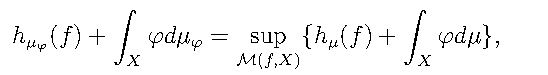
\includegraphics[width=6cm]{mathsnippet} & 
    
\includegraphics[width=5cm]{mathsnippet-libreoffice}\\\hline
  \end{tabular}
\caption{Copy \& Paste in Word Processors}\label{fig:cnp}
\end{figure}

There are several methods to transform papers from {\LaTeX} to an office word
processor. The first method is to just generate a PDF file and then open this file in
Word/LibreOffice. This achieves the goal of looking like the desired PDF document, just in
Office. There are two problems with this route: 
\begin{enumerate}
\item mathematical formulae are not preserved (see Figure~\ref{fig:cnp})
\item even if the result looks OK the results have lost their links (e.g. for
  citations/references or label/ref), or become difficult to edit, because they do not
  conform to the styling system of the word processor.
\end{enumerate}
The fundamental problem is that it converts the appearance of the document and loses
meaning due to macro expansion. This is especially blatant when looking at the math in a
document. Either it is treated as text, with no meaningful way to distinguish between math
and formatted text that happens to contain some mathematical symbols, making automatic
treatment of this kind of math difficult, or it is represented by an image of the relevant
formulae, which makes editing extremely impractical if not impossible. The same holds true
for references, they are essentially treated as parts of text with a linked number in
front of them, complicating adding new references substantially.

The other way of transforming {\LaTeX} to Word, by transforming the .tex file directly,
does away with some of these issues. Some editors to do this already exist, such as
TeX4ht~\cite{tex4ht:online}. This already does this admirably, however it is very focussed
on Libreoffice, e.g. it can't handle mathematics in docx files.

\section{Implementation}\label{sec:impl}

\begin{figure}[ht]\centering
\begin{tikzpicture}[yscale=1.5,xscale=1.2]
\tikzstyle{doc}=[draw,thick,align=center,color=black,
                 shape=document,minimum width=10mm,minimum height=8mm]
\node[doc] (p) at (-1,3.5) {\texttt{paper.tex}};
\node[doc] (b) at (1,3.5) {\texttt{group.bib}};
\node[doc,dashed] (px) at (-1,2.2) {\texttt{paper.ltxml}};
\node[doc,dashed] (bx) at (1,2.67) {\texttt{group.ltxml}};
\draw[->,thick] (p) -- node[left,near end] (l) {\latexml} (px);
\draw[->,thick] (b) -- (bx);
\draw[->,thick] (bx) -- (l);
\node[doc,dashed] (d) at (-2,1) {\texttt{document.xml}};
\node[doc,dashed] (r) at (0.2,1) {\texttt{relations.xml}};
\node[doc] (s) at (1,.3) {\texttt{styles.xml}};
\draw[->,thick] (px) -- node[left]{XSLT}(d);
\draw[->,thick] (px) -- node[right]{XSLT}(r); 
\node[inner sep=0pt,outer sep=0pt] (z) at (-1,.3) {};
\draw[thick] (d) -- (z);
\draw[thick] (r) -- (z);
\draw[thick] (s) -- (z);
\node[doc] (dx) at (0-1,-.4) {\texttt{paper.docx}};
\draw[->,thick] (z) -- node[left] {zip} (dx);
\draw[dotted] (-3.1,-.1) rectangle (1.9,1.9);
\node at (1.6,1.8) {post};
\end{tikzpicture}
\caption{The Transformation Process}\label{fig:arch}
\end{figure}

Both docx and odt files share a very similar structure and are almost interchangeable,
except for slight differences in syntax and different names. They both consist of zipped up XML files. The main content, such as text, placement of images, tables etc., is written in document.xml. The other important file is relations.xml, which contains information about where in the docx/odt file other supplementary files such as images are contained. Finally the archive contains various other objects such as style files, setting files and images. \\



To create the .odt/.docx files we first transform the .tex file to an intermediate
XML-based format using{\LaTeX}ml. \ednote{Papa Latexml erlaerung einfuegen}.

Then we use an XSLT stylesheet to generate document.xml from the .ltmxl file. For Word files, we use a Microsoft stylesheet to transform the MathML generated by {\LaTeX}ML to the docx math format. The other file we generate from the ltxml file using XSLT is relations.xml.The other supporting files such as images are placed into the correct file structure the postprocessor. As the penultimate step some static files, that don't change depending on the input document, are also placed into the correct directories.The main file of interest here is styles.xml, which contains the style information of the document. We had to create this ourselves to recreate the feel of the PDF files generated by {\LaTeX}. Finally the document is zipped to create the docx/odt file. \\ 


\ednote{Screenshot einfuegen}
\ednote{Bin eigentlich nicht zufrieden hiermit TT}

\section{Conclusion}\label{sec:concl}
We have presented a \latexml plugin that transforms {\LaTeX} papers into Word/Office
documents in a one-line system call. With the recent web front-end of \latexml, it will be
simple to extend this to a web service. The \latexml Word Processing plugin is public
domain and is available from GitHub at~\cite{LaTeX2Office:github:on}. The conversion makes
crucial use of the fact that \latexml preserves more of the document and formula semantics
than other systems that process \LaTeX documents, this ensures that the core process in
the transformation -- the translation of \latexml XML to Office XML (DOCX or ODF) has
enough information to generate the respective target document structures.

In the future we want to develop an office package for \LaTeX, which allows the direct
markup of higher-level structures -- e.g. document metadata in {\LaTeX} documents, so that
it can be transferred to the office documents. Similarly, we want to extend the
transformation to carry over even more semantics from the \stex format into semantically
extended office formats like CPoint or
CWord~\cite{Kohlhase:SemanticInteractionDesignDiss:biblatex}; this would finally give us a
way to cleanly interface the currently {\LaTeX}-based document methods in the KWARC group
to applied STEM disciplines.

\printbibliography
\end{document}



%  LocalWords:  maketitle ednote hline libreoffice includegraphics mathsnippet cnp Hier
%  LocalWords:  einen einfuegen glaube ich docx impl odt Latexml erlaerung eigentlich
%  LocalWords:  nicht zufrieden hiermit concl printbibliography
